\documentclass[a4paper,twoside]{article}

\usepackage{epsfig}
\usepackage{graphicx}
\usepackage{calc}
\usepackage{amssymb}
\usepackage{amstext}
\usepackage{amsmath}
\usepackage{amsthm}
\usepackage{multicol}
\usepackage{balance}
\usepackage{pslatex}
\usepackage{apalike}
\usepackage{algorithm2e}
\usepackage[bottom]{footmisc}
\usepackage{url}
\usepackage{tikz}
\usetikzlibrary{arrows.meta,positioning,shapes.geometric}
\usepackage{SCITEPRESS}

\begin{document}

\title{Instrumented VR Procedural Training for Smart Manufacturing: A Repeated-Measures Pilot Study of a Labeling Workstation}

% TODO for camera-ready: replace anonymous metadata with final authors, affiliations,
% ORCID identifiers and emails. Keep this anonymous for double-blind review.
\author{\authorname{Anonymous Authors}
\affiliation{Anonymous Institution}
\email{anonymous@anonymous.edu}}

\keywords{Virtual Reality, Digital Twin, Smart Factory, Industrial Training, Procedural Learning, Human-System Interface, Performance Evaluation.}

\abstract{Industrial training in smart factories requires repeatable, safe and measurable methods for acquiring procedural skills. This paper presents an instrumented immersive virtual reality training scenario developed within a broader smart-factory digital-twin project. The wider platform includes a connected supervision proof of concept that transmits a temperature measurement from a physical machine through ESP32 and FastAPI to Unity; the evaluated labeling scenario is a separate offline training module. It reproduces a nine-step industrial task and logs completion time, step-level timing and false-grab errors. A randomized within-subject pilot study with twelve participants evaluated three scene conditions together with workload, presence, comfort and acceptance. The primary question was whether the platform could detect repeated-exposure performance improvement while remaining usable and comfortable. Completion time decreased significantly across chronological exposure (Friedman $p=0.002$, Kendall's $W=0.53$), while acceptance and presence were high and VR symptoms were low. Error reduction and stress-condition effects were directionally promising but not statistically conclusive. The contribution is a measurement-capable immersive training module and a conservative pilot framework for human-centered digital-twin research.}

\onecolumn \maketitle \normalsize \setcounter{footnote}{0} \vfill

\section{\uppercase{Introduction}}
\label{sec:introduction}

Smart factories combine connected equipment, human operators, cyber-physical systems and real-time information flows. This evolution changes the role of training: operators must not only remember procedures but also execute them reliably, adapt to changing guidance and recover from interaction errors. Traditional training through written procedures, demonstrations or supervised observation remains valuable, but it is difficult to repeat under controlled conditions and rarely produces fine-grained behavioural data.

Immersive virtual reality (VR) can address this limitation by placing users in a controlled, repeatable and safe simulation of an industrial workstation. When connected conceptually or technically to a real production system, such environments can also support digital-twin training strategies \cite{Jones2020,Rasheed2020,Thelen2022}. However, a VR training system is scientifically valuable only if it goes beyond visual realism by supporting structured interaction and objective measurement of procedural performance.

This paper presents a pilot evaluation of an instrumented VR training platform for a smart-factory labeling workstation. The scenario reproduces a nine-step industrial procedure while recording completion time, step-level timing and false-grab errors. Objective logs are combined with subjective measures of workload, learning, presence, comfort, stress and acceptance to evaluate whether the platform can detect procedural improvement while remaining usable and comfortable.

This paper makes four contributions. First, it presents an instrumented VR procedural-training framework based on a finite-state interaction validator. Second, it introduces an event-logging architecture that records session- and step-level behavioural metrics. Third, it evaluates the framework through a randomized repeated-measures pilot study combining objective and subjective measures. Finally, it discusses how instrumented immersive environments can support future human-centered digital-twin research through reproducible behavioural evidence.

The proposed framework forms one component of a broader smart-factory digital-twin project. A connected supervision proof of concept acquires the extrusion-blow-molding machine temperature through an ESP32, transmits it via FastAPI and visualizes it in Unity. In contrast, the labeling scenario evaluated here operates as a standalone offline training module without controlling or synchronizing the physical workstation. Consequently, this paper evaluates the immersive training and behavioural measurement framework rather than the fidelity of the complete digital twin.

\section{\uppercase{Related Work}}
\label{sec:related}

\subsection{Digital Twins and Smart-Factory Training}

Recent reviews emphasize that digital twins should be understood through their data connections, physical-to-virtual updates, virtual-to-physical interpretation and lifecycle purpose rather than as static three-dimensional models \cite{Jones2020,Rasheed2020,Thelen2022}. Human-centered manufacturing research further positions operator interaction, workload, ergonomics and safety as explicit digital-twin concerns \cite{Wilhelm2021,Berti2022}. For educational smart-factory environments, this perspective is valuable because it links process representation, interaction and measurement. A training platform can therefore be evaluated not only by visual realism, but also by the quality of the data it produces for understanding user performance.

\subsection{Immersive VR for Procedural Industrial Learning}

Immersive VR has been widely investigated for learning and training because it supports embodied interaction, safe repetition and exposure to scenarios that may be costly or risky in the physical environment \cite{Radianti2020,Radhakrishnan2021,Tusher2024}. A review of process-industry operator training found that only 10 of 44 studies compared immersive and conventional training and identified time, mistakes and hints as recurring effectiveness indicators \cite{Fracaro2022}. A recent procedural-training meta-analysis reported an overall positive medium effect, while also identifying substantial heterogeneity in interventions, terminology and outcome measurement \cite{Jongbloed2024}. Experimental manufacturing studies have compared virtual and physical robot operation \cite{Monetti2022}, while procedural-training research has examined VR against conventional instruction and alternative learning strategies \cite{DeLorenzis2023}. These studies show the value of objective outcomes, but they also leave room for compact, instrumented platforms that expose within-subject learning trajectories and step-level diagnostic data.

\begin{center}
\centering
\captionof{table}{Positioning against recent VR training research.}
\label{tab:positioning}
\scriptsize
\setlength{\tabcolsep}{3pt}
\renewcommand{\arraystretch}{1.18}
\vspace{1mm}
\begin{tabular}{p{1.45cm}p{1.25cm}p{2.55cm}}
\hline
\textbf{Study} & \textbf{Design} & \textbf{Primary contribution}\\
\hline
Fracaro et al. (2022) & Review & Training indicators and comparative-evidence gap\\
\hline
Monetti et al. (2022) & Between-mode & VR versus physical robot performance\\
\hline
De Lorenzis et al. (2023) & Comparative & Instruction mode and procedural retention\\
\hline
This study & Repeated measures & Runtime validation, event logs and exposure trajectories\\
\hline
\end{tabular}
\end{center}

\subsection{Guidance, Autonomy and Measurement}

In a VR procedure, guidance cues can support the first exposure, whereas later unguided execution can reveal whether the user has internalized the sequence. The Cognitive Affective Model of Immersive Learning links immersion and control to presence, agency, cognitive load and procedural learning outcomes \cite{Makransky2021}. Recent XR theory likewise treats presence, plausibility and congruence as important but insufficient descriptors of user experience \cite{Latoschik2021}. Subjective experience therefore has to be interpreted alongside objective outcomes such as completion time and interaction errors. This paper treats subjective measures as feasibility and construct indicators, while total time and false grabs are the main behavioural endpoints.

\section{\uppercase{System Design}}
\label{sec:system}

\subsection{Role within the Digital-Twin Project}

Unlike many VR industrial-training applications that primarily emphasize visualization, the proposed system was designed as an instrumented experimental platform. The architecture combines procedural state validation, behavioral event logging and immersive interaction so that every user action can be objectively analyzed. Within the broader smart-factory project, the labeling workstation represents the human-training component, while the connected supervision module demonstrates the integration pathway with physical industrial data.

The connected supervision path and the offline training path share the same virtual representation of the production environment, but only the supervision proof of concept currently consumes physical data. The labeling scenario contributes the interaction, procedural-control and human-performance layers of the broader project.

\subsection{Training Scenario}

The prototype is a standalone VR scenario deployed in Unity for a Meta Quest-class headset. The virtual workstation reproduces an industrial labeling task in which the user manipulates bins, bottles and labels, follows a prescribed sequence and validates the final label placement. Figure~\ref{fig:environment_sequence} illustrates the workstation, instruction display and label-placement interaction. The task is represented as a nine-step procedure. Each step has a target action, and the system can activate guidance elements such as visual cues, spatial indicators and audio instructions.

\begin{center}
    \centering
    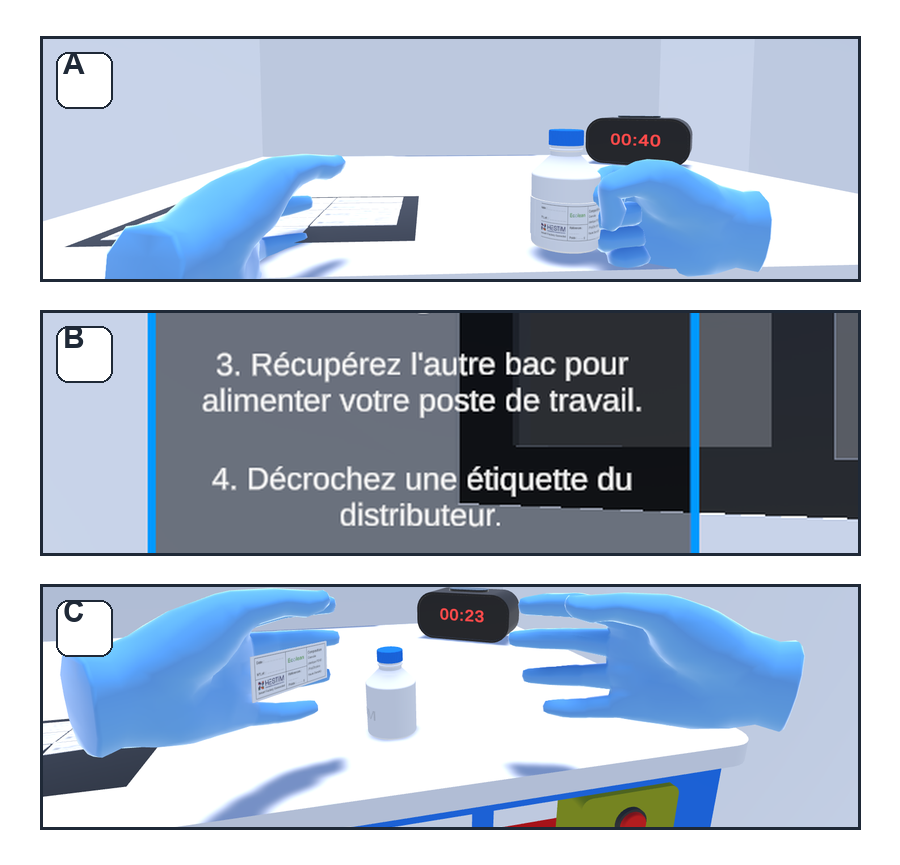
\includegraphics[width=\linewidth]{figures/fig_environment_sequence.png}
    \captionof{figure}{Representative views of the immersive labeling scenario: workstation manipulation, procedural guidance display and label-placement interaction.}
    \label{fig:environment_sequence}
\end{center}

\subsection{Instrumentation and Data Logging}

The system architecture was organized around a finite-state procedural controller rather than a passive visual simulation. Let $S_i$ denote the active procedural step and $e=(o,a,t)$ an interaction event containing the selected object, action and timestamp. A step-specific guard $g_i(e)$ evaluates whether the event matches the expected object--action pair. If $g_i(e)=1$, the logger records the elapsed step time and the controller advances to $S_{i+1}$; otherwise, it records a false grab and retains $S_i$. Figure~\ref{fig:controller} formalizes this validation loop. The scene condition configures cue availability without changing the rule, so every accepted and rejected interaction remains interpretable against the prescribed procedure.

The system logs objective data at the session level and at the procedural-step level. The primary objective endpoint is total completion time in seconds. Secondary objective endpoints are step-level completion times and false-grab counts. A false grab is counted when the user attempts to interact with an object that is not valid for the current procedural state. This metric is intended to capture hesitation, object-selection errors and interaction ambiguity. This instrumentation layer transforms the virtual environment into a measurement platform rather than a passive simulation. By preserving both procedural-state information and detailed interaction events, the framework enables quantitative analyses of learning progression, procedural bottlenecks and interaction quality, providing behavioral evidence that extends beyond traditional completion-time measurements.

\begin{center}
    \centering
    \resizebox{\linewidth}{!}{%
    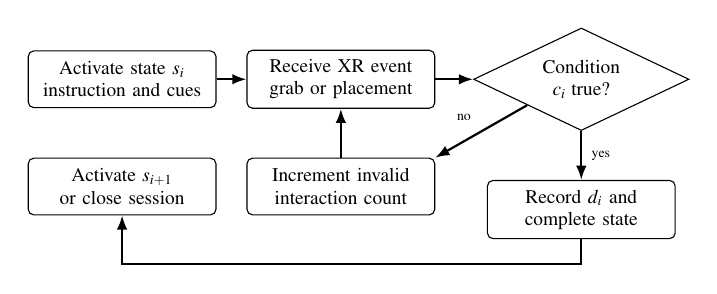
\begin{tikzpicture}[
        state/.style={draw=black, fill=white, text=black, rounded corners=2pt, text width=2.15cm, minimum height=0.72cm, align=center, font=\scriptsize},
        decision/.style={diamond, draw=black, fill=white, text=black, aspect=2.1, align=center, font=\scriptsize},
        data/.style={draw=black, fill=white, text=black, rounded corners=2pt, text width=2.15cm, minimum height=0.72cm, align=center, font=\scriptsize},
        arrow/.style={-{Latex[length=1.8mm]}, thick}
    ]
    \node[state] (activate) {Activate state $s_i$\\instruction and cues};
    \node[state, right=0.38cm of activate] (event) {Receive XR event\\grab or placement};
    \node[decision, right=0.48cm of event] (valid) {Condition\\$c_i$ true?};
    \node[data, below=0.62cm of event] (invalid) {Increment invalid\\interaction count};
    \node[data, below=0.62cm of valid] (record) {Record $d_i$ and\\complete state};
    \node[state, left=0.38cm of invalid] (next) {Activate $s_{i+1}$\\or close session};
    \draw[arrow] (activate) -- (event);
    \draw[arrow] (event) -- (valid);
    \draw[arrow] (valid) -- node[right,font=\tiny] {yes} (record);
    \draw[arrow] (record.south) -- ++(0,-0.32cm) -| (next.south);
    \draw[arrow] (valid.south west) -- node[above left,font=\tiny] {no} (invalid.north east);
    \draw[arrow] (invalid) -- (event);
    \end{tikzpicture}%
    }
    \captionof{figure}{State transition and interaction-validation logic. Invalid actions are observable but do not advance the procedure.}
    \label{fig:controller}
\end{center}

\section{\uppercase{Experimental Protocol}}
\label{sec:protocol}

\subsection{Participants and Design}

Twelve participants completed the pilot study. Their mean age was 21.2 $\pm$ 3.0 years (range 19--30); ten were male and two were female. Seven participants were enrolled in Industrial Engineering (GI) and five in Computer Engineering (GIN). Ten reported that this was their first VR experience, whereas two reported previous VR experience. All participants performed three VR sessions, yielding 36 retained objective records and 36 matched questionnaire condition blocks. One questionnaire row identified as a pilot/test entry was excluded before analysis. Because the female and VR-experienced subgroups each contained only two participants, demographic subgroup comparisons were treated as descriptive and were not used for inferential claims.

The design is within-subject. Each participant completed all three scene conditions: guided execution, autonomous execution and a stress-test condition. The observed scene order was randomized across participants, but the realized allocation was not fully balanced after the first exposure. Run 1 contained four participants in each condition; Run 2 contained five guided, six autonomous and one stress session; Run 3 contained three guided, two autonomous and seven stress sessions. The analysis therefore separates chronological run effects from scene-condition effects, while acknowledging that the two factors are not orthogonal in this pilot. Run 1, Run 2 and Run 3 are used to evaluate repeated-exposure improvement, while condition labels are used to examine condition-related burden.

\subsection{Procedure and Data Handling}

The experiment was conducted as a supervised repeated-exposure session. Participants received the task objective, headset safety instructions and interaction conventions, then completed three executions of the same nine-step procedure. The guided condition emphasized instructional cues, the autonomous condition reduced assistance and the stress-test condition introduced a more demanding variant. The same state validator was active in all conditions, so accepted events, rejected interactions and timing variables were logged using a common rule. Objective logs and questionnaires were joined by anonymized participant and session/condition labels; one row marked as a pilot/test entry was removed before analysis. Because the study was a pilot rather than a preregistered trial, feasibility thresholds and exploratory correlations are interpreted as analytic benchmarks.

\subsection{Subjective Measures}

The post-session questionnaire contained workload, perceived-performance, learning/autonomy, presence/realism, VR-symptom, guidance/adaptation, stress and acceptance items. Composite scores were unweighted means of available items; no item was reverse-scored. Workload and perceived performance used 0--10 scales, learning/autonomy, guidance/adaptation, stress and acceptance used 1--5 scales, presence/realism used 1--7 and symptoms used 0--3. Descriptive internal consistency across the 36 session blocks was acceptable for workload ($\alpha=.82$), learning/autonomy ($\alpha=.85$), presence/realism ($\alpha=.72$), symptoms ($\alpha=.76$) and acceptance ($\alpha=.84$), but lower for guidance/adaptation ($\alpha=.65$). These coefficients describe the present adapted instrument and do not constitute independent scale validation.

\subsection{Hypotheses}

Based on the reframed research question, the pilot evaluates five expectations: H1, procedural efficiency should improve with repeated VR exposure; H2, interaction errors should decrease as users stabilize procedural and motor control; H3, the platform should be feasible for immersive industrial training, reflected in high acceptance, high presence/realism and low symptoms; H4, the stress-test condition should produce measurable objective burden without unacceptable discomfort; and H5, presence/realism may be associated with objective performance accuracy. These expectations are not treated equally in the interpretation: H1 and H3 are central, whereas the stress and correlation analyses are exploratory in the current pilot.

\subsection{Statistical Analysis}

Given the small sample and repeated-measures structure, non-parametric tests were used. Omnibus differences across three repeated conditions were evaluated using the Friedman rank test. Pairwise contrasts used exact Wilcoxon signed-rank tests, with Holm adjustment within each pairwise family. The eight subjective-composite omnibus tests were additionally treated as one exploratory family and Holm-adjusted across scales. Effect sizes are reported as Kendall's $W$ for Friedman tests, rank-biserial correlation ($r_{\mathrm{rb}}$) for signed-rank contrasts and Spearman's $\rho$ for exploratory correlations. Paired standardized mean differences are used only as secondary descriptive quantities where helpful.

Because chronological run and scene condition were imbalanced, a sensitivity model was fitted to log completion time and $\log(1+\text{false grabs})$, with participant fixed effects and indicator terms for run and condition. Partial $F$ statistics were evaluated with 5,000 within-participant permutations, preserving each participant's three outcomes while disrupting their run--condition assignment. Correlations used participant averages and 100,000 deterministic permutations; three reported relationships were Holm-adjusted as one exploratory family. Figures emphasize raw observations and mean $\pm$ SD.

\section{\uppercase{Results}}
\label{sec:results}

\subsection{Primary Endpoint: Completion Time}

The strongest result is the chronological learning signal in completion time. As summarized in Figure~\ref{fig:learning_results}, mean total time decreased from 101.1 $\pm$ 41.1 s in Run 1 to 65.6 $\pm$ 31.0 s in Run 2 and 67.5 $\pm$ 34.5 s in Run 3. The repeated-measures effect was significant, $\chi^2(2)=12.67$, $p=0.002$, Kendall's $W=0.53$. Pairwise contrasts showed significant reductions from Run 1 to Run 2 (raw $p=0.002$, Holm $p=0.005$, $r_{\mathrm{rb}}=-0.92$) and from Run 1 to Run 3 (raw $p<0.001$, Holm $p=0.001$, $r_{\mathrm{rb}}=-1.00$). Run 2 and Run 3 did not differ ($p=0.677$).

The adjusted sensitivity model supported the same interpretation. After controlling for scene condition and participant, chronological run explained log completion time (partial $F=15.73$, permutation $p<0.001$), whereas scene condition did not (partial $F=1.44$, $p=0.261$). Relative to Run 1, adjusted log-time coefficients were $-0.437$ for Run 2 and $-0.455$ for Run 3. This robustness check reduces, but does not eliminate, concern that the observed learning curve was produced by the realized condition order.

\begin{figure}[!t]
    \centering
    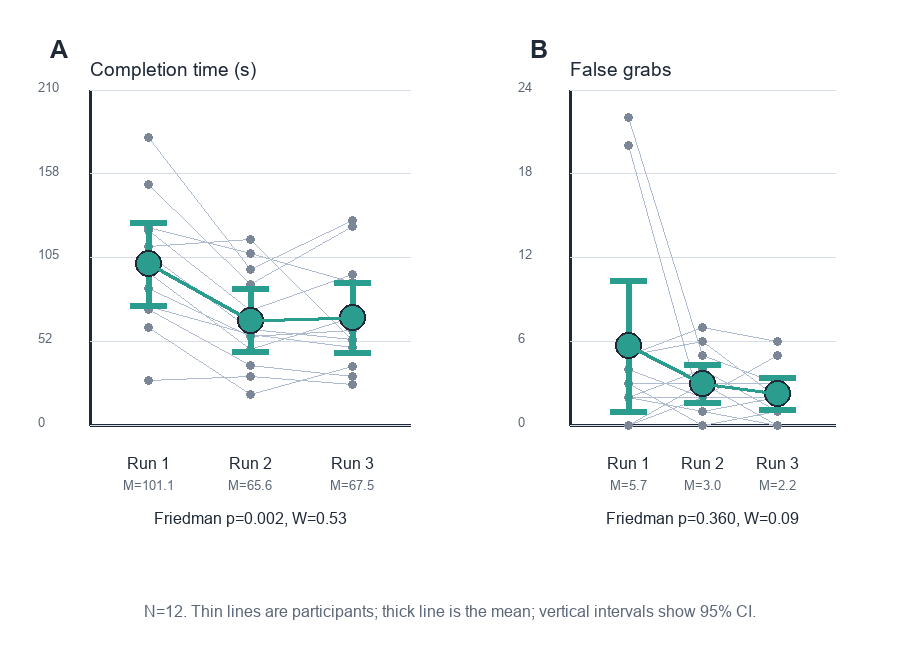
\includegraphics[width=\linewidth]{figures/fig_session_learning_spaghetti.png}
    \caption{Learning curves across chronological exposure. Thin lines show individual participants, the thick line shows the group mean and vertical intervals show 95\% confidence intervals.}
    \label{fig:learning_results}
\end{figure}

\subsection{Secondary Endpoint: False Grabs}

False-grab counts decreased descriptively from 5.7 $\pm$ 7.4 in Run 1 to 3.0 $\pm$ 2.1 in Run 2 and 2.3 $\pm$ 1.8 in Run 3. However, the omnibus Friedman test was not significant, $\chi^2(2)=2.04$, $p=0.360$, Kendall's $W=0.09$. No pairwise contrast remained significant; the largest reduction, from Run 1 to Run 3, had raw $p=0.102$ and Holm-adjusted $p=0.305$. Therefore, H2 is interpreted as directional support rather than a confirmed effect.

\subsection{Condition Effects}

The stress-test condition was descriptively slower and more error-prone than the guided condition. Mean completion time was 72.4 $\pm$ 34.8 s in the guided condition, 78.6 $\pm$ 38.5 s in the autonomous condition and 83.2 $\pm$ 44.1 s in the stress condition. Mean false grabs were 2.9 $\pm$ 1.9, 2.7 $\pm$ 2.0 and 5.3 $\pm$ 7.5, respectively. Figure~\ref{fig:condition_statistics} displays the participant-level distributions behind these summaries. However, condition effects were not significant for completion time ($p=0.472$, Kendall's $W=0.06$) or false grabs ($p=0.979$, Kendall's $W<0.01$). The stress result is therefore useful as a design signal, but it should not be presented as a confirmed experimental effect.

\begin{figure}[!t]
    \centering
    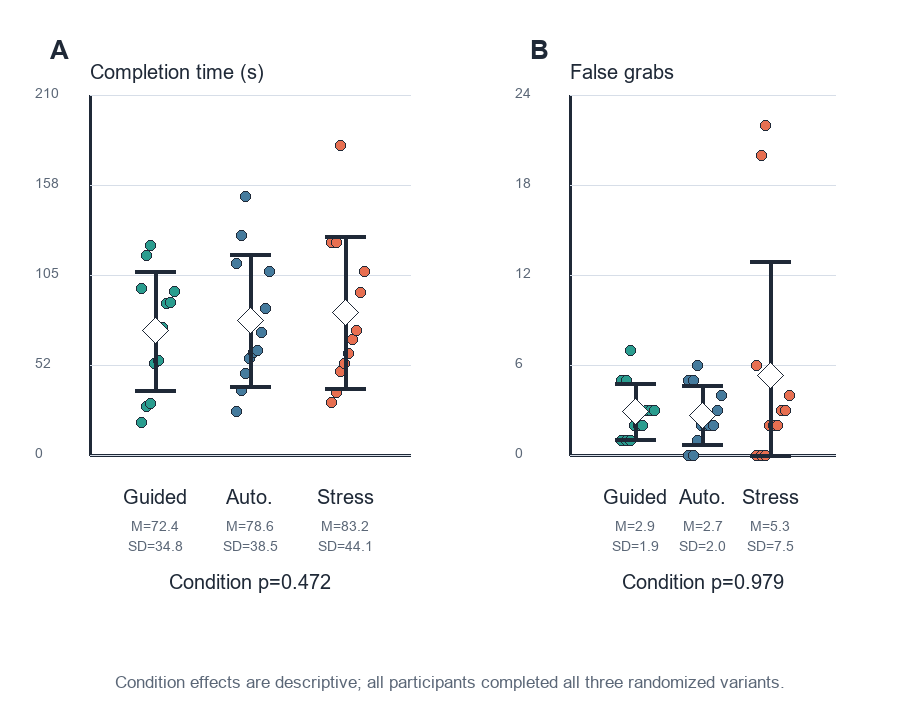
\includegraphics[width=\linewidth]{figures/fig_condition_statistics.png}
    \caption{Exploratory condition-level distributions. The stress variant shows higher mean burden, but condition effects were not statistically significant in the current pilot.}
    \label{fig:condition_statistics}
\end{figure}

\subsection{Step-Level Diagnostic Profile}

The exported step times were used as a descriptive diagnostic layer rather than as the primary timing endpoint. Five records differed by more than one second between total completion time and the sum of exported step times, and the first and final validation steps were approximately zero in the log. For this reason, the step profile is interpreted cautiously. It nevertheless shows what the instrumentation can reveal beyond a single total-time measure. Figure~\ref{fig:step_diagnostics} shows that the strongest reduction from Run 1 to Run 2 was concentrated in early and mid-procedure steps, especially Step 2, Step 4 and Step 6. False-grab errors were also concentrated in a small number of steps during the first exposure and became less prominent in later runs. This pattern suggests that future versions should preserve step-level logging and add event-severity markers, because the diagnostic value lies in identifying where procedural uncertainty emerges.

\begin{figure}[!t]
    \centering
    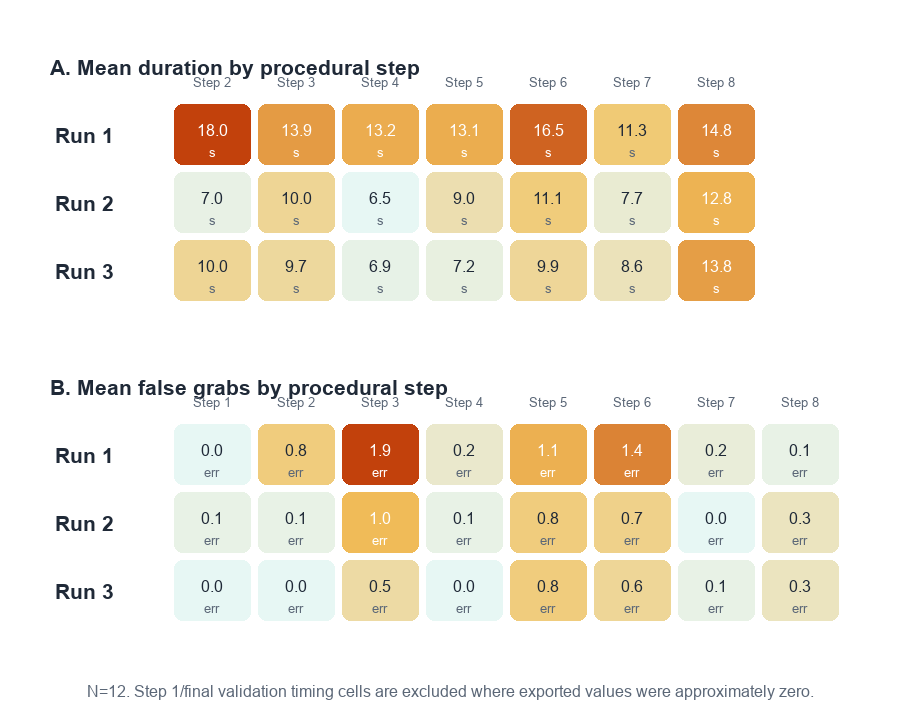
\includegraphics[width=\linewidth]{figures/fig_step_session_heatmap.png}
    \caption{Step-level diagnostic profile across chronological exposure. Mean duration and mean false-grab counts are shown for each exported procedural step, allowing the sources of global improvement to be localized.}
    \label{fig:step_diagnostics}
\end{figure}

\subsection{Subjective Feasibility}

Subjective responses supported the feasibility of the platform. Across participant-level averages, global acceptance was 4.85 $\pm$ 0.29 on a 1--5 scale, presence/realism was 6.51 $\pm$ 0.47 on a 1--7 scale and VR symptoms were 0.38 $\pm$ 0.36 on a 0--3 scale. Exact one-sample signed-rank tests showed that acceptance was above an interpretive high-feasibility benchmark of 4/5 ($p=0.001$), presence/realism was above 5/7 ($p<0.001$) and symptoms were below a mild-symptom benchmark of 1/3 ($p=0.001$). Figure~\ref{fig:subjective_statistics} shows chronological subjective trends after aligning the questionnaire blocks to the objective session order. The subjective profile remained stable: workload stayed low, perceived performance and acceptance stayed high and symptoms remained close to the floor. These findings support H3.

Learning/autonomy produced the smallest unadjusted condition-level p-value among the eight subjective composites, $\chi^2(2)=9.04$, nominal $p=0.011$, Kendall's $W=0.38$. Mean scores increased from 4.33 $\pm$ 0.79 in the guided condition to 4.90 $\pm$ 0.11 in the autonomous condition and 4.96 $\pm$ 0.10 in the stress condition. However, the omnibus result did not survive Holm adjustment across the eight composites ($p_{\mathrm{Holm}}=0.087$). Within-scale pairwise values (autonomous versus guided $p_{\mathrm{Holm}}=0.033$; stress versus guided $p_{\mathrm{Holm}}=0.012$) are therefore descriptive follow-ups rather than confirmatory effects. The pattern may reflect perceived independence after guidance, but ceiling effects further limit its precision.

\begin{figure}[!t]
    \centering
    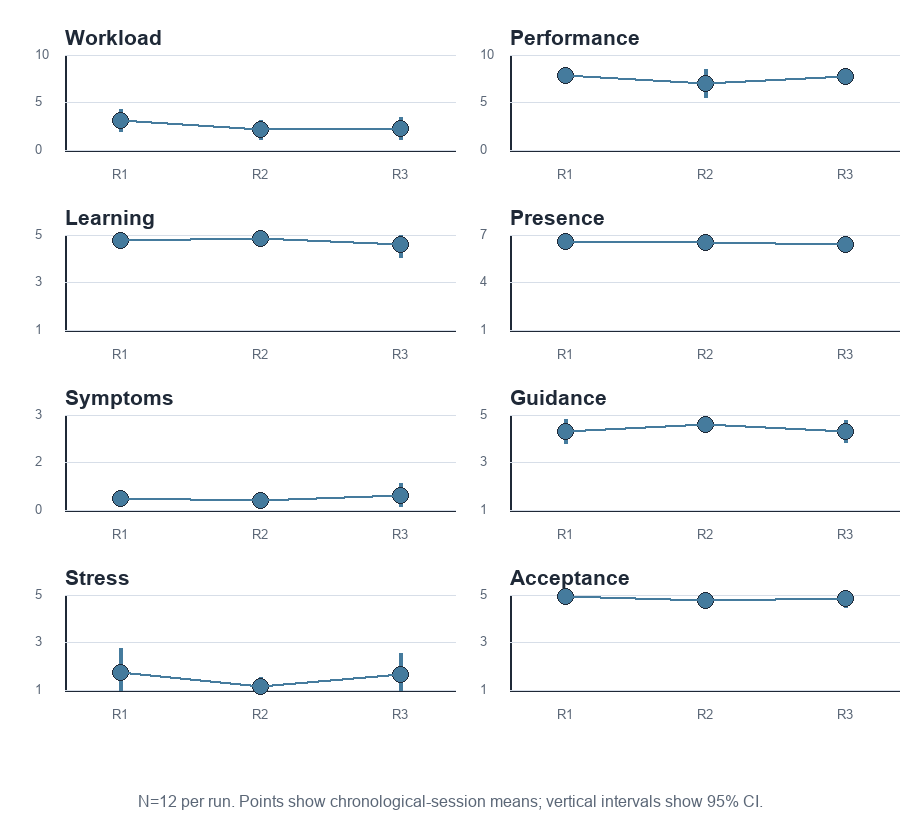
\includegraphics[width=\linewidth]{figures/fig_subjective_session_multiples.png}
    \caption{Subjective scale trends across chronological exposure. Each panel reports the group mean with 95\% confidence intervals on the original scale of the corresponding construct.}
    \label{fig:subjective_statistics}
\end{figure}

\subsection{Subjective--Objective Relationships}

The exploratory association between presence/realism and objective accuracy was not supported. Participant-average Spearman correlations were $\rho=-0.08$ for false grabs ($p=0.796$) and $\rho=-0.12$ for completion time ($p=0.698$). Workload showed a positive association with completion time ($\rho=0.59$, nominal $p=0.046$), but this did not survive Holm adjustment across the three relationships ($p_{\mathrm{Holm}}=0.138$). Figure~\ref{fig:participant_relationships} therefore presents these results as candidate relationships for a larger study, with participants rather than sessions as the analysis unit.

\begin{figure}[!b]
    \centering
    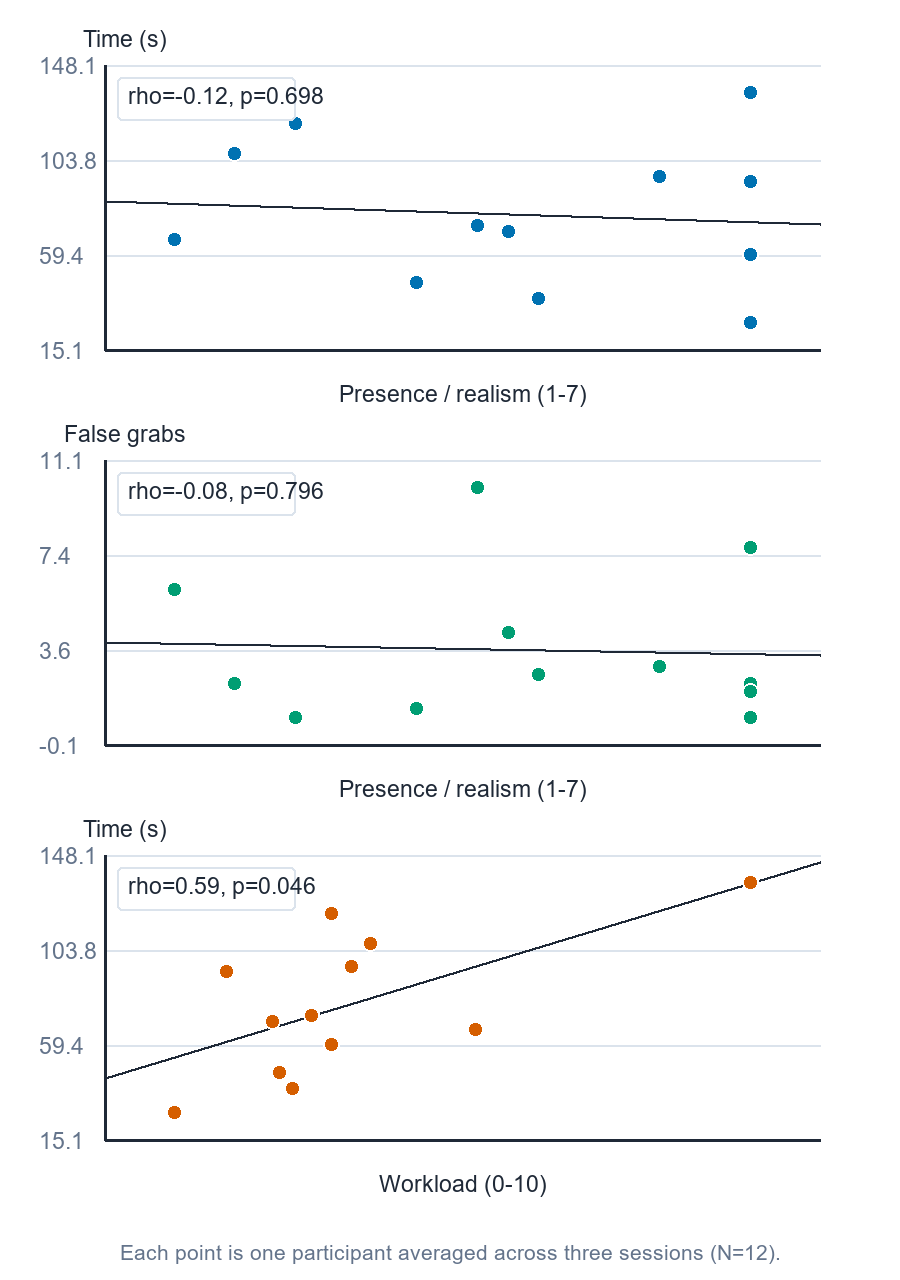
\includegraphics[width=0.92\linewidth]{figures/fig_participant_relationships.png}
    \caption{Participant-level subjective--objective relationships ($N=12$). Points are participant averages across three sessions; displayed p-values are unadjusted permutation values and none survived Holm correction across the three panels.}
    \label{fig:participant_relationships}
\end{figure}

The mixed pattern of results is best interpreted as pilot evidence rather than as a definitive training trial. The data provide strong support for repeated-exposure efficiency gains and subjective feasibility, directional but underpowered support for error reduction, an exploratory stress-condition signal and no support for a presence-performance association in this sample.

\section{\uppercase{Discussion}}
\label{sec:discussion}

The main scientific value of the pilot is not that the VR system was positively perceived, but that it produced measurable behavioural evidence. Completion time showed a large and statistically significant within-subject improvement from the first exposure to subsequent runs. This supports the claim that the environment is sensitive to repeated-exposure improvement, which may combine procedural learning, interface familiarization and motor adaptation. In a conference context focused on informatics, control, automation and human-system interfaces, the measurement architecture is part of the technical contribution because it connects runtime procedural control with analyzable behavioural logs.

The step-level profile also illustrates why an instrumented VR task can be more informative than an overall score alone. Although the step-time data are not treated as primary inferential endpoints in this pilot, they reveal plausible bottlenecks associated with chronological exposure and procedural uncertainty. This diagnostic layer is important for future digital-twin training research: it can guide scenario redesign, identify confusing instructions and support targeted adaptation of guidance rather than merely reporting whether a participant finished faster or slower.

The subjective results complement the behavioural findings. High acceptance and presence/realism, together with low symptom scores, suggest that the platform is usable enough for repeated experimental exposure. This comfort result matters because cybersickness remains a recognized barrier to sustained HMD use and requires explicit evaluation rather than assumption \cite{Ang2023}. The learning/autonomy pattern is compatible with greater perceived independence after guidance, but it did not survive correction across the questionnaire family and should not be generalized. The feasibility findings, supported by acceptable consistency for most multi-item composites, remain the stronger secondary contribution.

The stress-test condition should be interpreted more cautiously. Although the stress condition was descriptively slower and more error-prone, the pilot sample was small and the condition effect was not statistically significant. In addition, no independent event-severity log was available. Future versions should log which unexpected event occurred, its timing and its severity. This would allow stress or disruption to be evaluated as an experimental manipulation rather than only as a scene label.

Presence/realism did not predict performance. This may reflect a true absence of association, but it may also be caused by ceiling effects: most participants rated presence and acceptance highly, leaving little variance for correlation. Future work should include a larger and more diverse sample, possibly with a more sensitive validated presence scale.

\section{\uppercase{Threats to Validity}}
\label{sec:validity}

The study is a pilot with twelve participants, so inferential results should be interpreted conservatively. The sample was demographically imbalanced, with only two female participants and two participants with previous VR experience; the study was not powered to test gender, academic-program or VR-experience moderation. The realized condition order was also imbalanced after Run 1. The participant-adjusted permutation model showed that the run effect survived statistical control for condition, but this post hoc adjustment cannot provide the protection of a fully counterbalanced design. Five retained objective records differed by more than one second between total completion time and the sum of exported step times, so total completion time was treated as the primary timing endpoint. False-grab counts also showed high variability.

The subjective questionnaire was adapted for this pilot. Internal consistency was acceptable for most composites, but guidance/adaptation was weaker and several constructs showed ceiling effects. Future work should use validated scale translations where possible, preregister missing-data and feasibility rules and report consent, recruitment and ethics procedures in the camera-ready documentation.

Another limitation concerns the absence of an external comparison group. The current design can show within-subject improvement across VR exposure, but it cannot prove superiority over written instructions, video training or physical demonstration. A future ICINCO-oriented extension should compare VR against at least one conventional training baseline, include delayed retention and stratify allocation by academic program and previous VR experience.

Finally, the experiment does not validate the complete digital-twin architecture. The connected subsystem was demonstrated on one physical temperature measurement, while the labeling scenario ran offline and did not receive live workstation states or send control commands to the production line. The results therefore concern the immersive training and measurement layer; they do not establish synchronization fidelity, predictive capability or bidirectional control.

\section{\uppercase{Conclusions}}
\label{sec:conclusion}

This paper presented an instrumented immersive VR scenario developed as the training component of a broader smart-factory digital-twin project and evaluated it in a randomized within-subject pilot study. Its finite-state validator generated objective behavioural logs and step-level diagnostic information. Completion time decreased across repeated exposure, and this effect remained after participant-level adjustment for scene condition. The platform also showed high acceptance and presence with low symptom scores. Error reduction, condition differences and subjective--objective associations were not statistically conclusive after appropriate multiplicity control. The study therefore validates the sensitivity and feasibility of the offline measurement module, not training superiority or the full connected twin. Future work should add a conventional-training baseline, delayed retention, full counterbalancing and live physical-state integration.

% TODO for camera-ready if accepted:
% Add acknowledgements, funding, conflict-of-interest, data-sharing and AI-tool statements according to SCITEPRESS/INSTICC requirements.

\bibliographystyle{apalike}
\balance
{\small
\bibliography{paper}}

\end{document}
